El IP (Internet Protocol) es un protocolo de la capa de Red (capa 3) que contiene información de direccionamiento y cierta información de control que permite enrutar los paquetes. Envía y recibe bloques de datos llamados datagramas, recibidos del software de la capa superior. Fue inventado en 1974 ( Vint Cerf and Bob Kahn). \\${ }$\\
Proporciona un servicio de distribución de paquetes de información \textbf{orientado a no conexión} de manera no fiable. La orientación a no conexión significa que los paquetes de información, que seran emitidos a la red, son tratados independientemente, pudiendo viajar por diferentes trayectorias para llega a su destino. El término no fiable significa mas que nada que no se garantiza la recepción del paquete.
\subsubsection*{Direcciones IP}
\subsubsection*{\texttt{IPv4} y \texttt{IPv6}}
\begin{itemize}
\item \texttt{IPv4}: Fue la primera versión de IP. Fue implementado para la producción del ARPANET en 1983. Es la versión IP mas utilizada. Utiliza un esquema de direcciones de 32 bits que permite almacenar $2^{32}$ direcciones (4 mil millones).
\item \texttt{IPv6}: Es la siguiente versión de IP. Internet Engineer Taskforce la inició a principios del 94. Su objetivo era resolver los problemas asociados a \texttt{IPv4}. Con un espacio de direcciones de 128 Bits. Tambien se le llama \texttt{IPng} (IP next generation).
\end{itemize}

\subsection*{Datagrama}

\begin{figure}[H]                           
\centering                                  
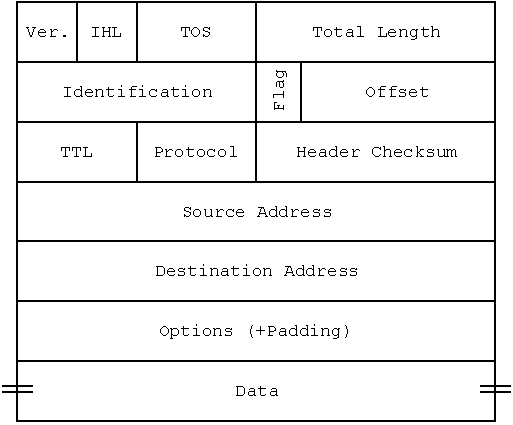
\includegraphics[page=1,scale=0.85]{IP.pdf}
\end{figure}                

\begin{itemize}
\item \texttt{Version} (4Bits): Numero de version del protocolo IP.
\item \texttt{IHL, Internet Header Length }(4Bits): Longitud del encabezado expresados en el numero de grupos.
\item \texttt{TOS, Type of Service} (8Bits): Se utiliza para indicar la prioridad o importancia de los datos enviados.
\item \texttt{Total Length} (16Bits): Es la longitud en bytes del datagrama completo, incluyendo el encabezado y los datos. (Encabezado + Datos). Tamaño máximo: $2^{16}$.
\item \texttt{Identification} (16Bits): Se utiliza para facilitar el ensamble de las fragmentos del datagrama.
\item \texttt{Flag} (3Bits):
\begin{itemize}
\item \texttt{DF (Dont Fragment)}: Sirve para identificar paquetes que no se pueden fragmentar.
\item \texttt{MF (More Fragment)}: Sirve para identificar paquetes que se pueden fragmentar. \texttt{MF} esta en 1 cuando aun hay fragmentos que están llegando al datagrama original, y es 0 cuando es el ultimo.
\item \texttt{RS (Reservado)}: Debe ser 0 si o si.
\end{itemize}
\item \texttt{Offset} (13Bits):  Desplazamiento de fragmento. En paquetes fragmentados indica la posición que ocupa el paquete en el datagrama original. Por lo tanto el primer paquete tiene este valor como 0.
\item \texttt{TTL, Time To Live} (8Bits): Contiene un número que disminuye cada vez que el paquete pasa por un nodo. Si llega a 0 se descarta para evitar que los paquetes sigan en la red. (128 Usualmente)
\item \texttt{Protocol} (8Bits): Indica el protocolo. Es decir el paquete que viene detrás (por ejemplo si es TCP).
\item \texttt{Checksum} (16Bits): Necesario para verificar que los datos contenidos en el encabezado son correctos.
\item \texttt{Source Address} (32BBits): Usuario que envía el paquete.
\item \texttt{Destination Address} (32Bits): Dirección del usuario que recibe la información.
\item \texttt{Options}: No es obligatorio y tiene dos posibles formatos: Opciones Simples y Compuestas.
\item \texttt{Padding}: Se asegura que el header termina en 32bits añadiendo ceros hasta que se hace múltiplo de 32.
\end{itemize}                
$\bigstar$ IPv4 e IPv6 no son compatibles no tienen la misma trama.            
                
\subsection*{Fragmentación}         
Es un mecanismo que permite separar o fragmentar un datagrama IP en diversos bloques llamados ``fragmentos'' , si su tamaño sobrepasa la Unidad Máxima de Transferencia (\texttt{MTU}). El protocolo IP solamente fragmenta un datagrama cuando la \texttt{MTU} del medio por donde se encamina tiene un tamaño menor que el datagrama.     
                
%\begin{figure}[H]
%\centering
%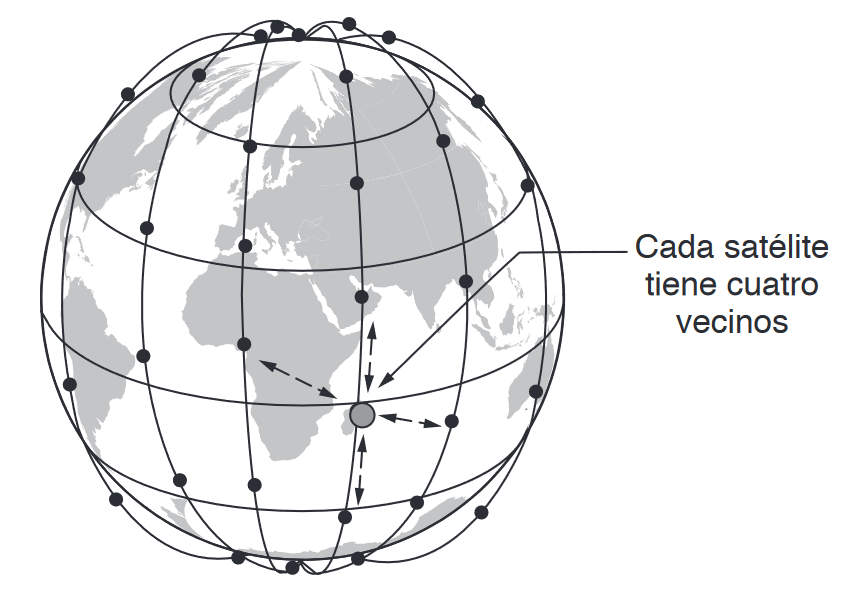
\includegraphics[page=1,scale=0.7]{SATELITES2.png}
%\caption{Satélites Iridium \textit{(Redes de Computadoras, Tanenbaum 4ta Edición, Pagina 105)}}
%\end{figure}

%\begin{figure}[H]
%\centering
%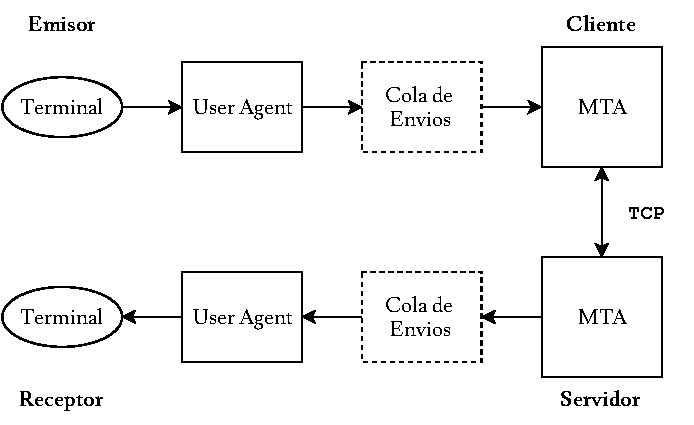
\includegraphics[page=1,scale=0.7]{SMTP.pdf}
%\caption{Esquema de funcionamiento de SMTP}
%\end{figure}
